\documentclass[a4paper,10pt]{article}

\usepackage{ucs}
\usepackage[utf8x]{inputenc}
\usepackage{amsmath}
\usepackage{amssymb}
\usepackage{subfigure}
\usepackage[german]{babel}
\usepackage{fontenc}
\usepackage{graphicx}
\usepackage{capt-of}
\usepackage{natbib}
\bibliographystyle{apj.bst}
\usepackage{aas_macros}

\usepackage[dvips]{hyperref}

\date{03/15/15}

\begin{document}
 \section{Introduction}
 --Initial Problem (graph of obs data)\\
 --First thoughts (Hypothesis)\\
 \section{Method}
 --Which Method did I use and why?\\
 \textbf{For this approach I used two programs: main.py and lumiradius.py.} \\
 
 I had the choice between two different approaches: A montecarlo approach and a grid approach. \\
 
 In my program I use the grid approach. I span a grid in distance-mass-age. The range of these three
 variables can be easily adjusted, as can the binning. In accordance to the observational data I try to explain, distance goes from \
 0 to $r_{max}=3kpc$. Mass will also be in the same parameters, as the observational data:
 from $M_{min}=5M_\odot$ to $M_{max}=50M_\odot$. The mass-distribution will follow the Salpeter Initial Mass Function (IMF)\citep[see][]{1955ApJ...121..161S}.
 Because the IMF follows an inverse power law, I use a logarithmic mass-grid.\\
 Age can be implemented in two different ways: I could either use a seperate age-axis for every star going from 0 to $t_{ms}(M)$ or I can
 use a single axis for all stars spanning from 0 to $t_{ms}(M_{min})$. Because the main sequence age ($t_{ms}$) of a star 
 is a strictly monotonic increasing function of M $t_{ms}(M_{min})=t_{max}$. \textbf{I use the second approach}. With $M_{min}=5M_\odot$ this 
 translates to $t_{max}=104Myr$. This Axis will also be logarithmic to make sure massive stars with small $t_{ms}$ are correctly
 represented. \\
 The three informations I have about any given star, are its mass, its age and its distance from earth. From these three informations
 I need to derive its fractional main sequence age ($\tau$), its apparent magnitude (V) and ultimately the probability density
 for all stars.\\ 
 First I will implement a stellar evolution model by \citet*{2000MNRAS.315..543H} which approximates the stellar evolution as a 
 function of initial mass ($M_{ini}$), fractional main sequence age ($\tau$) and metalicity(Z). \\
 To do this, first I need to find a function for $\tau$. Using equation 5 \citep[page 547]{2000MNRAS.315..543H} I know the main sequence age 
 ($t_{ms}$) and $\tau$ then becomes: $\tau=\frac{t}{t_{ms}}$. Since I only include stars on the main sequence, I can safely include
 the condition: $\tau<1$ to cut down on computing time.
 Equation 12 and 13 from the same paper are very powerful equations to compute luminosity and radius for a star on the main sequence.\\
 This Paper does reference \citet*{1996MNRAS.281..257T} for Zero Age Mainsequence (ZAMS) Radii and Luminosities. However there is one 
 error in this Paper I had to correct. In Equation 1 $\gamma + M^3$ has to be $\gamma \cdot M^3$.\\
 \textbf{insert HRD illustrating lumiradius}\\
 
 The program does allow for freely changeable metalicities. For my purposes I use Z=0.02 for all stars to simulate
 a metalicity similar to that of our galactic neighborhood.\\
 I now run this program for every possible mass-age tuple and save the results in a matrix. This way I don't have to call the program for
 every distance-mass-age triple and massively cut down on computing time.\\
 With all this I now know distance, mass, age, fractional main sequence age, luminosity and radius for any given star. I can now use these 
 informations to compute the apparent magnitudes.
 \begin{equation}
  M_{V}=V-5\cdot\log_{10}(distance)+5-Red
  \label{MV}
 \end{equation}
 \begin{equation}
  M_{bol}=M_{V}+BC
  \label{Mbol}
 \end{equation}
 \begin{equation}
  \frac{L}{L_\odot}=0.4\cdot(4.72-M_{bol})
  \label{LMbol}
 \end{equation}
 Where $M_{V}$ is the absolute visual magnitude, Red is the reddening as a function of distance, $M_{bol}$ is the absolute bolometric 
 magnitude and BC is the Bolometric Correction. Using equations \ref{MV}, \ref{Mbol} and \ref{LMbol} I can now compute the apparent visual
 magnitude V:
 \begin{equation}
  V=5\cdot\log_{10}(distance)-5+Red+4.72-\frac{L}{L_\odot\cdot0.4}-BC
 \end{equation}
 To get a rough approximation for reddening, I use \citet*[Figure 9]{2005AJ....130..659A} and interpolate between these values 
 1:0.9, 2:2.25 and 3:3.273\\
 The next thing I need to know are the probability densities for stars in space $\left(\frac{dp}{dV}\right)$, mass 
 $\left(\frac{dp}{dm}\right)$ and age $\left(\frac{dp}{dt}\right)$. In my simulation I assume a homogenous distribution of stars. 
 This makes finding a probability density for space very easy. Because of the radial symmetry of my problem the distribution becomes
 solely dependant on the distance from earth:
 \begin{equation}
  \frac{dp}{dV}=\frac{1}{V_{tot}}=\frac{1}{\frac43\cdot\pi\cdot maxdistance^3}
  \label{dpdV}
 \end{equation}
 I assume a constant star formation rate, so the probability density in age would be similar to the density in distance. I do however use
 a logarithmic binning in age. Thus I can not simply use $\frac{dp}{dt}$ but instead need to find $\frac{dp}{d\log t}$ using the following:
  $\frac{dp}{dt}=\frac{1}{t_{ms}}\quad \land \quad d\log t=\frac{dt}{t \ln 10}$
 \begin{equation}
  \frac{dp}{d\log t}=\frac{t\ln 10}{t_{ms}}
 \end{equation}
 I assume, that the stars are distributed in mass following the Salpeter IMF:
 $\frac{dp}{dM}=A\cdot M^{-2.35}$\citep{1955ApJ...121..161S}. Similar
 to the density function in age, I need to convert it for my logarithmic binning using $dlogM = \frac{dM}{M\ln 10}$
 \begin{equation}
  \frac{dp}{d\log M}=\ln 10 \cdot A\cdot M^{-1.35}
 \end{equation}
 Where A is a normalization factor, that needs to be computed. 
 \begin{equation}
  1=\int_{M_{min}}^{M_{max}}A\cdot M^{-2.35} dM =\left[ -1.35\cdot A\cdot M^{-1.35}\right]_{M_{min}}^{M_{max}}
 \end{equation}
 \begin{equation}
  A= \frac{1.35}{M_{min}^{-1.35}-M_{max}^{-1.35}}
 \end{equation}
 With this information I can now formulate an overarching probability density function with regard to $\tau$
 \begin{equation}
  \frac{dp}{d\tau}=\frac{dp}{dV}dV \cdot \frac{dp}{d\log t}d\log t \cdot \frac{dp}{d\log M}d\log M\cdot \frac{1}{d\tau}
 \end{equation}
 I now split $\tau$ in 20 bins. For every possible star in my sample I will check $\tau\le 1$ and $V\le 9$ This way I count every
 star on the main sequence, that falls below my magnitude cut. 

 
 The binning can be freely adjusted. To optimize runtime of my program I conducted a few tests to adjust the binnings in all three dimensions.\\
 \section{testing stuffs}
 I 
  \begin{center}
  \begin{minipage}{0.49\textwidth}
   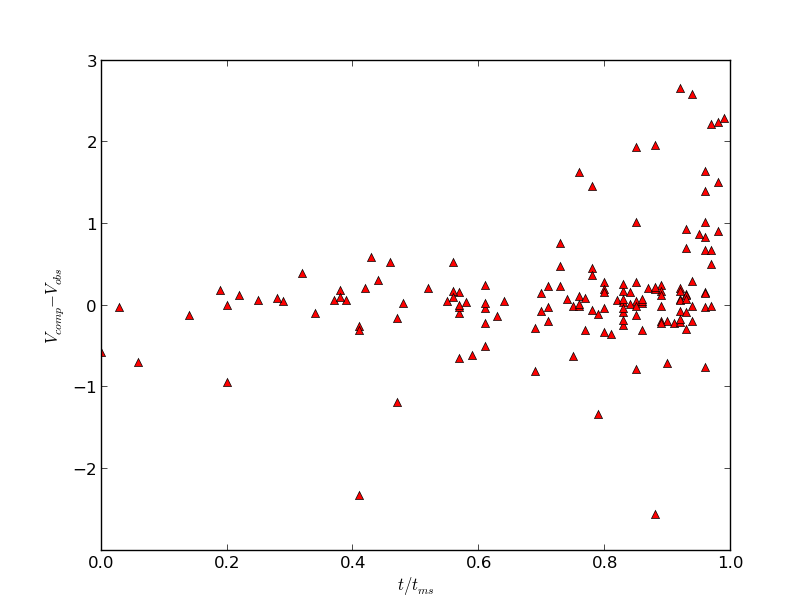
\includegraphics[width=\textwidth]{diffmagfracms}
  \end{minipage}
  \begin{minipage}{0.49\textwidth}
   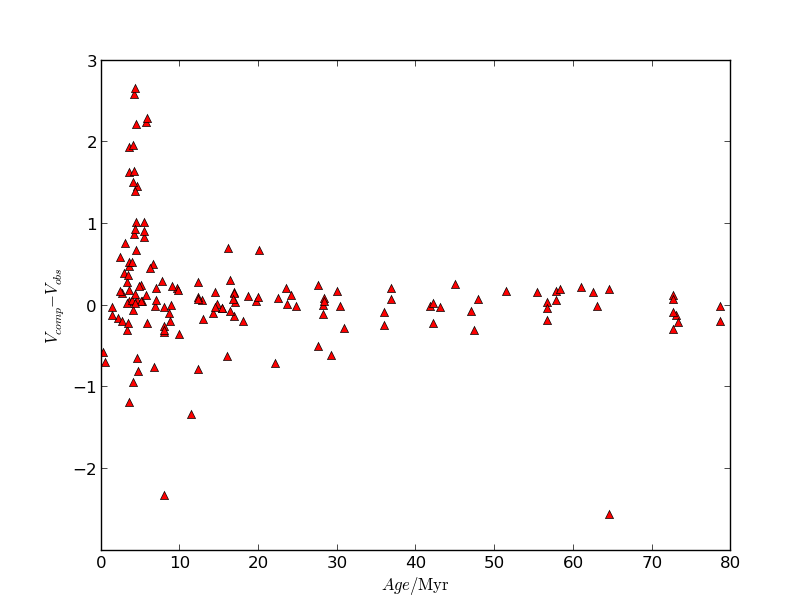
\includegraphics[width=\textwidth]{diffmagAge}
  \end{minipage}
 \end{center}
 \captionof{figure}{Difference between computed and observed magnitudes as a function of fractional main sequence age (left) and total age
 (right). The theoretical magnitudes were computed using stellar radius, luminosity and distance.\label{fracageage}}
 
 
 Figure \ref{fracageage} shows the difference between computed and observed magnitudes as a function of fractional main sequence age (left) and total age
 (right). It shows, that for some stars there is an offset to higher $V_{comp}$ at high $\tau$ and low absolute ages. This implies, that
 this disagreement shows up in high-mass stars near TAMS. This can be explained using \citep[figure 1]{2014A&A...570L..13C}. My code uses
 an evolutionary model similar to the one used at the lefthand side. $V_{obs}$ however is obtained using a model similar to the righthand
 side. Because TAMS is shifted in the righthand side, there will be differences at TAMS.
 
 \begin{center}
  \begin{minipage}{0.49\textwidth}
   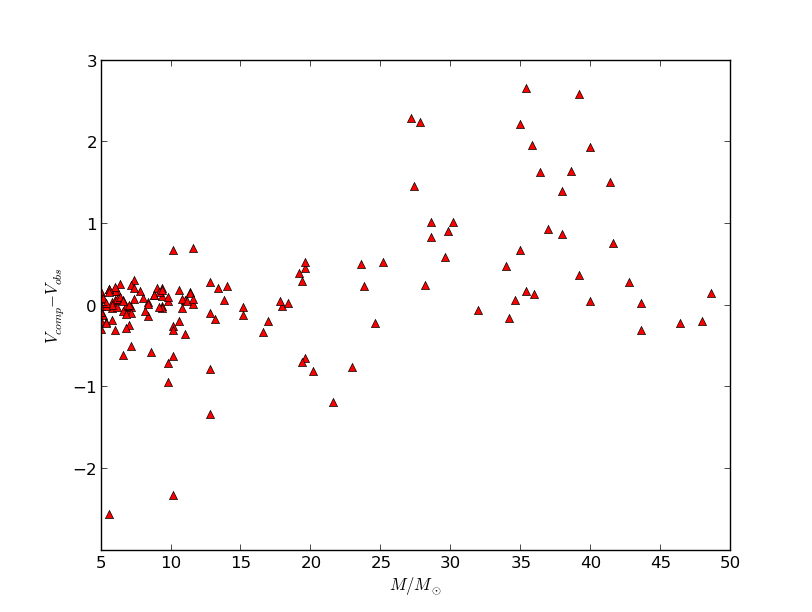
\includegraphics[width=\textwidth]{diffmagmass}
  \end{minipage}
  \begin{minipage}{0.49\textwidth}
   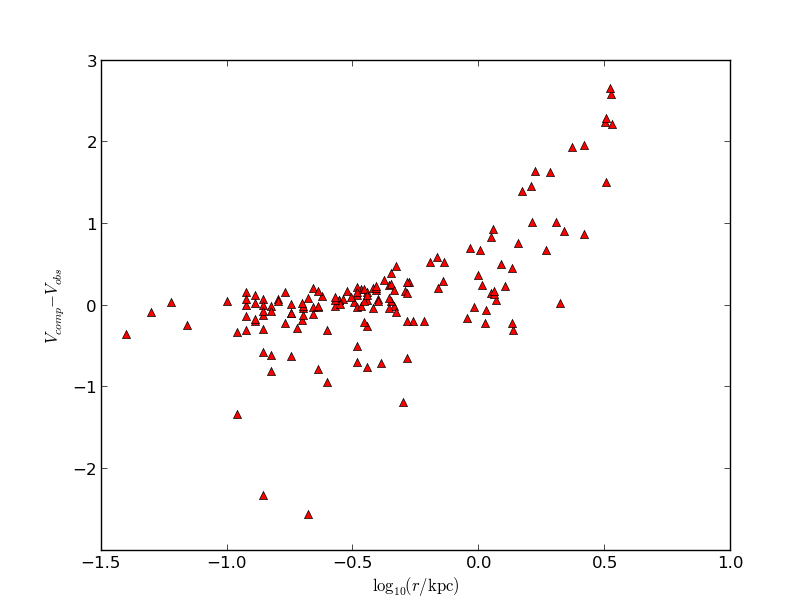
\includegraphics[width=\textwidth]{diffmaglogdist}
  \end{minipage}
 \end{center}
 \captionof{figure}{Difference between computed and observed magnitudes as a function of Mass (left) and $log_{10}(distance)$ (right).
 The theoretical magnitudes were computed using stellar radius, luminosity and distance. \label{massdist}}
 
 Figure \ref{massdist} 
 
 
 \begin{center}
  \begin{minipage}{0.49\textwidth}
   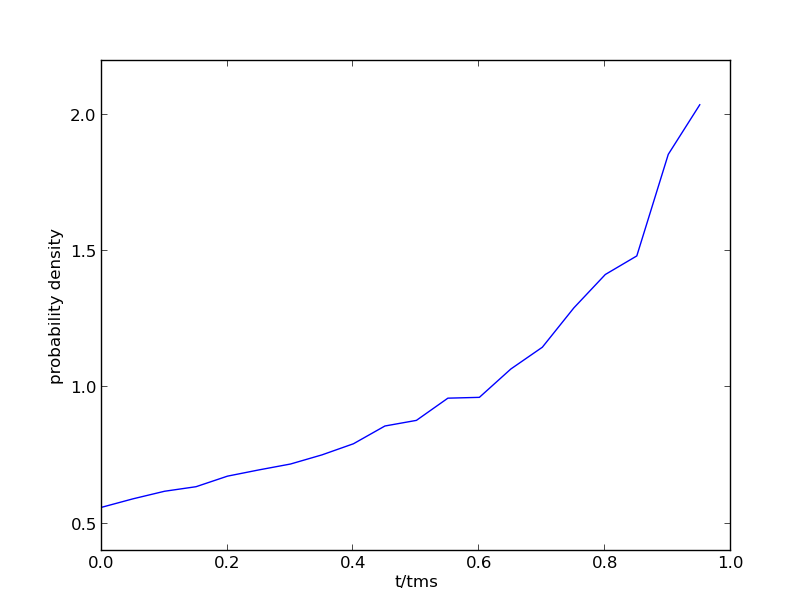
\includegraphics[width=\textwidth]{100-100-100}
  \end{minipage}
  \begin{minipage}{0.49\textwidth}
   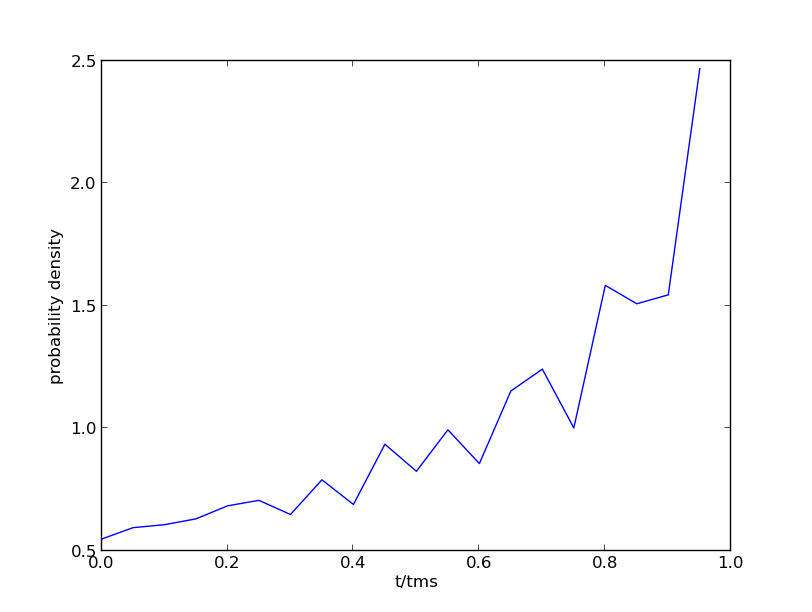
\includegraphics[width=\textwidth]{50-50-50}
  \end{minipage}
   \captionof{figure}{Probability density function for all stars in my sample with a magnitude cut at V=9 with binnings of
 100-100-100 (left) and 50-50-50 (right) in distance-mass-age.\label{100-100-100}}
 \end{center}

 \begin{center}
  \begin{minipage}{0.49\textwidth}
   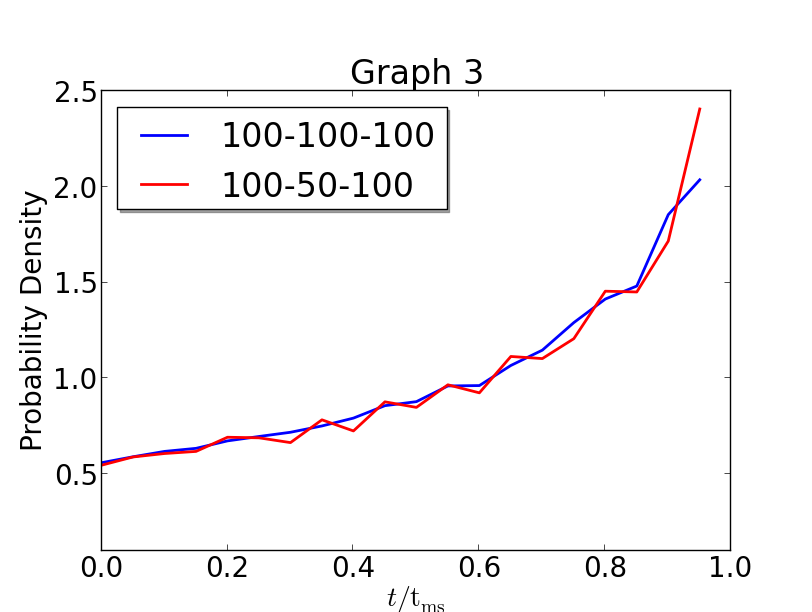
\includegraphics[width=\textwidth]{100-50-100}
  \end{minipage}
  \begin{minipage}{0.49\textwidth}
   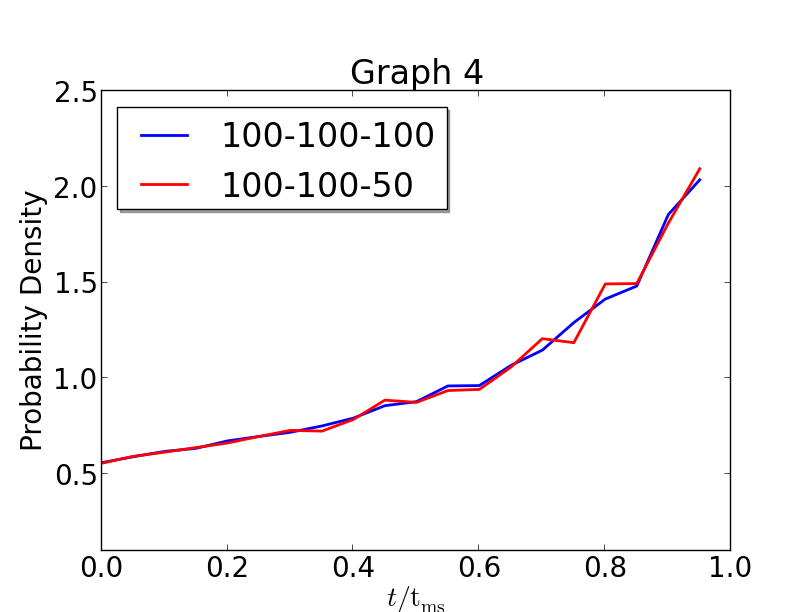
\includegraphics[width=\textwidth]{100-100-50}
  \end{minipage}
   \captionof{figure}{Probability density function for all stars in my sample with a magnitude cut at V=9 with binnings of
 100-50-100 (left) and 100-100-50 (right) in distance-mass-age.\label{100-50-100}}
 \end{center}

 
 
 \begin{center}
  \begin{minipage}{0.49\textwidth}
   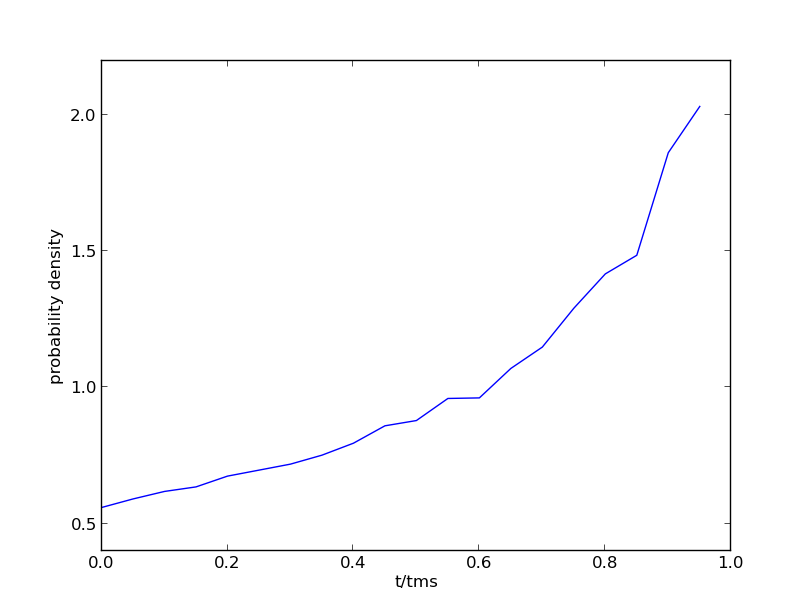
\includegraphics[width=\textwidth]{50-100-100}
  \end{minipage}
  \begin{minipage}{0.49\textwidth}
   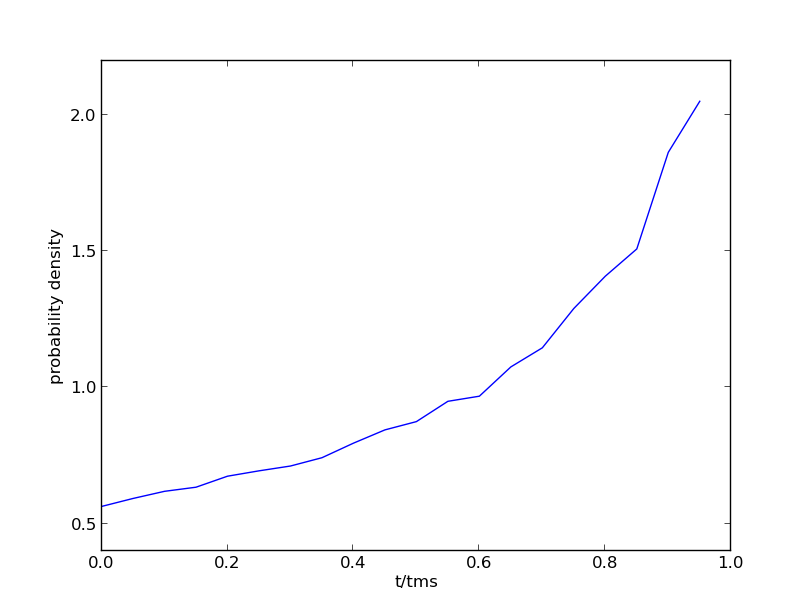
\includegraphics[width=\textwidth]{10-100-100}
  \end{minipage}
   \captionof{figure}{Probability density function for all stars in my sample with a magnitude cut at V=9 with binnings of
 50-100-100 (left) and 10-100-100 (right) in distance-mass-age.\label{10-100-100}}
 \end{center}
 
 
 
 \section{ending}
 
 \bibliography{adssample}
\end{document}
